\chapter{PENGUJIAN DAN ANALISIS}
\label{chap:pengujiananalisis}

% Ubah bagian-bagian berikut dengan isi dari pengujian dan analisis

Pada bab ini dipaparkan hasil pengujian serta analisa dari desain sistem dan implementasi. Pengujian dilakukan guna mengetahui tingkat kesalahan dan menarik kesimpulan dari sistem yang telah dibuat.

Pada proses pengujian digunakan salah satu layanan \textit{Google} yaitu \textit{Google Colaboratory} dengan spesifikasi \textit{hardware} seperti pada Tabel \ref{tab:spek-colab}. Sedangkan untuk spesifikasi \textit{hardware} komputer penulis dapat dilihat pada Tabel \ref{tab:spek-pc}.
\begin{table}[h]
	\begin{center}
		\begin{tabular}{ |c|c| } 
			\hline
			\textbf{Procesor} & Intel Xeon Processor @ 2.3 GHz\\
			\hline 
			\textbf{Graphic Card} & Tesla K80 12 GB GDDR5 VRAM\\
			\hline 
			\textbf{RAM} & 16 GB\\ 
			\hline
		\end{tabular}
		\caption{Spesifikasi \textit{hardware Google Colaboratory}}
		\label{tab:spek-colab}
	\end{center}
\end{table} 

\begin{table}[h]
	\begin{center}
		\begin{tabular}{ |c|c| } 
			\hline
			\textbf{Procesor} & Intel(R) Core(TM) i5-10400F CPU @ 2.90GHz\\
			\hline 
			\textbf{Graphic Card} & Nvidia GeForce GTX 1650 4 GB GDDR6\\
			\hline 
			\textbf{RAM} & 8 GB\\ 
			\hline
		\end{tabular}
		\caption{Spesifikasi \textit{hardware} Komputer yang Digunakan}
		\label{tab:spek-pc}
	\end{center}
\end{table}

Pengujian dilakukan dengan membagi model ke beberapa jenis \textit{backbone} yang digunakan, antara lain Resnet-50, Resnet-101, dan Mobilenet-V1.

\section{Pengujian Jenis \textit{Backbone}}
\label{sec:pengujian-backbone}

Pengujian pada jenis \textit{backbone} bertujuan untuk mengetahui performa dan akurasi dari setiap model yang dihasilkan dengan \textit{backbone} yang berbeda.

\subsection{Resnet-50}
\label{subsec:resnet50}

Tabel \ref{tab:conf-resnet50} merupakan parameter-parameter yang digunakan untuk membuat model Mask R-CNN dengan menggunakan \textit{backbone} Resnet-50.

\begin{longtable}[h]{|l|l|}
		\hline
		\multicolumn{2}{|c|}{\textbf{Pengaturan Model Resnet-50}}                                                                                                                                                                         \\ \hline
		BACKBONE                        & resnet50                                                                                                                                                                              \\ \hline
		BACKBONE\_STRIDES               & {[}4, 8, 16, 32, 64{]}                                                                                                                                                                 \\ \hline
		BATCH\_SIZE                     & 1                                                                                                                                                                                      \\ \hline
		BBOX\_STD\_DEV                  & {[}0.1 0.1 0.2 0.2{]}                                                                                                                                                                  \\ \hline
		COMPUTE\_BACKBONE\_SHAPE        & None                                                                                                                                                                                   \\ \hline
		DETECTION\_MAX\_INSTANCES       &	 50                                                    	\\ \hline
		IMAGE\_META\_SIZE               & 16                                                                                                                                                                                     \\ \hline
		IMAGE\_MIN\_DIM                 & 400                                                                                                                                                                                    \\ \hline
		IMAGE\_MIN\_SCALE               & 0                                                                                                                                                                                      \\ \hline
		IMAGE\_RESIZE\_MODE             & square                                                                                                                                                                                 \\ \hline
		IMAGE\_SHAPE                    & {[}512 512{]}                                                                                                                                                                             \\ \hline
		LEARNING\_MOMENTUM              & 0.9                                                                                                                                                                                    \\ \hline
		LEARNING\_RATE                  & 0.001                                                                                                                                                                                  \\ \hline
		LOSS\_WEIGHTS                   & \begin{tabular}[c]{@{}l@{}}\{'rpn\_class\_loss': 1.0, \\ 'rpn\_bbox\_loss': 1.0, \\ 'mrcnn\_class\_loss': 1.0, \\ 'mrcnn\_bbox\_loss': 1.0, \\ 'mrcnn\_mask\_loss': 1.0\}\end{tabular} \\ \hline
		MASK\_POOL\_SIZE                & 14                                                                                                                                                                                     \\ \hline
		MASK\_SHAPE                     & {[}28, 28{]}                                                                                                                                                                           \\ \hline
		MAX\_GT\_INSTANCES              & 50                                                                                                                                                                                     \\ \hline
		MEAN\_PIXEL                     & {[}123.7 116.8 103.9{]}                                                                                                                                                                \\ \hline
		MINI\_MASK\_SHAPE               & (56, 56)                                                                                                                                                                               \\ \hline
		NAME                            & object                                                                                                                                                                                 \\ \hline
		NUM\_CLASSES                    & 4                                                                                                                                                                                      \\ \hline
		POOL\_SIZE                      & 7                                                                                                                                                                                      \\ \hline
		MASK\_SHAPE                     & {[}28, 28{]}                                                                                                                                                                           \\ \hline
		MAX\_GT\_INSTANCES              & 50                                                                                                                                                                                     \\ \hline
		MEAN\_PIXEL                     & {[}123.7 116.8 103.9{]}                                                                                                                                                                \\ \hline
		MINI\_MASK\_SHAPE               & (56, 56)                                                                                                                                                                               \\ \hline
		NAME                            & object                                                                                                                                                                                 \\ \hline
		NUM\_CLASSES                    & 4                                                                                                                                                                                      \\ \hline
		POOL\_SIZE                      & 7                                                                                                                                                                                      \\ \hline
		POST\_NMS\_ROIS\_INFERENCE      & 1000                                                                                                                                                                                   \\ \hline
		POST\_NMS\_ROIS\_TRAINING       & 2000                                                                                                                                                                                   \\ \hline
		PRE\_NMS\_LIMIT                 & 6000                                                                                                                                                                                   \\ \hline
		ROI\_POSITIVE\_RATIO            & 0.33                                                                                                                                                                                   \\ \hline
		RPN\_ANCHOR\_RATIOS             & {[}0.5, 1, 2{]}                                                                                                                                                                        \\ \hline
		RPN\_ANCHOR\_SCALES             & (32, 64, 128, 256, 512)                                                                                                                                                                \\ \hline
		RPN\_ANCHOR\_STRIDE             & 1                                                                                                                                                                                      \\ \hline
		RPN\_BBOX\_STD\_DEV             & {[}0.1 0.1 0.2 0.2{]}                                                                                                                                                                  \\ \hline
		RPN\_NMS\_THRESHOLD             & 0.7                                                                                                                                                                                    \\ \hline
		RPN\_TRAIN\_ANCHORS\_PER\_IMAGE & 256                                                                                                                                                                                    \\ \hline
		STEPS\_PER\_EPOCH               & 100                                                                                                                                                                                    \\ \hline
		TOP\_DOWN\_PYRAMID\_SIZE        & 256                                                                                                                                                                                    \\ \hline
		TRAIN\_BN                       & False                                                                                                                                                                                  \\ \hline
		TRAIN\_ROIS\_PER\_IMAGE         & 200                                                                                                                                                                                    \\ \hline
		USE\_MINI\_MASK                 & True                                                                                                                                                                                   \\ \hline
		USE\_RPN\_ROIS                  & True                                                                                                                                                                                   \\ \hline
		VALIDATION\_STEPS               & 30                                                                                                                                                                                     \\ \hline
		WEIGHT\_DECAY                   & 0.0001  
		\\ \hline 
	\caption{Konfigurasi Model menggunakan Resnet-50 }
	\label{tab:conf-resnet50}
\end{longtable}

Setelah dilakukan serangkaian proses training yang memakan waktu sekitar 3 jam 40 menit 24 detik didapatkan \textit{output} berupa \textit{model file}  dengan format \textit{h5} yang mempunyai ukuran 170.9 MB. \textit{Training loss} terendah yang berhasil dicapai dengan menggunakan \textit{backbone} Resnet-50 (pada \textit{epoch} ke 242) adalah 0.4061 dengan rincian \textit{training bounding box loss} sebesar 0.04083, \textit{training classification loss} sebesar 0.02268 serta \textit{training mask loss} sebesar 0.139 (dimana $L=L_{bbox}+L_{cls}+L_{mask}$). Gambar \ref{fig:resnet50-training} merupakan grafik yang menunjukkan perubahan \textit{training loss, training bounding box loss, training classification loss,} serta \textit{training mask loss} dari \textit{epoch} 1 sampai 300.

\begin{figure}[h]
	\centering
	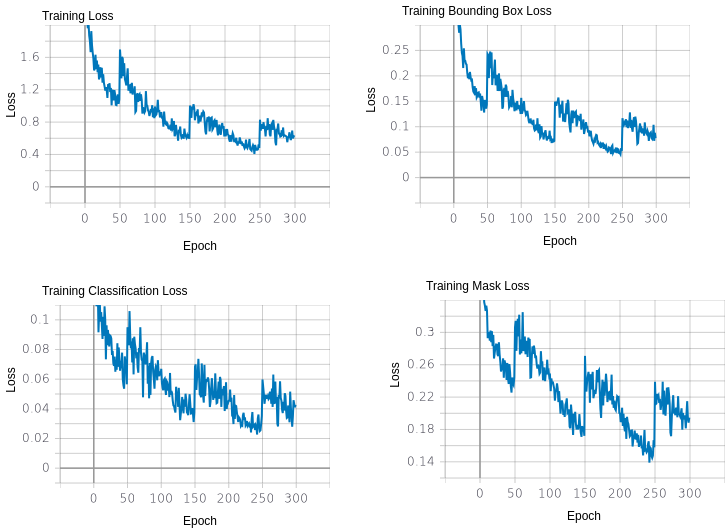
\includegraphics[scale=0.36]{gambar/resnet50-training.png}
	\caption{Grafik Perubahan \textit{Training Loss} pada Resnet-50}
	\label{fig:resnet50-training}
\end{figure}

Sedangkan pada saat proses \textit{validation} sendiri \textit{Loss} terendah yang berhasil dicapai pada \textit{epoch} ke 266 dengan nilai sebesar 0.3653 dengan rincian \textit{validation bounding box loss} sebesar 0.4556, \textit{validation classification loss} sebesar 0.01912 serta \textit{validation mask loss} sebesar 0.1519. Namun untuk \textit{validation bounding box loss} terendah berada pada \textit{epoch} ke 260 dengan nilai sebesar 0.4203 sedangkan \textit{validation classification loss} terendah pada \textit{epoch} ke 210 dengan nilai 0.01525 serta \textit{validation mask loss} terendah pada \textit{epoch} ke 201 dengan nilai 0.1439. Gambar \ref{fig:resnet50-val} merupakan grafik yang menunjukkan perubahan \textit{validation loss, validation bounding box loss, validation classification loss,} serta \textit{validation mask loss} dari \textit{epoch} 1 sampai 300.

\begin{figure}[h]
	\centering
	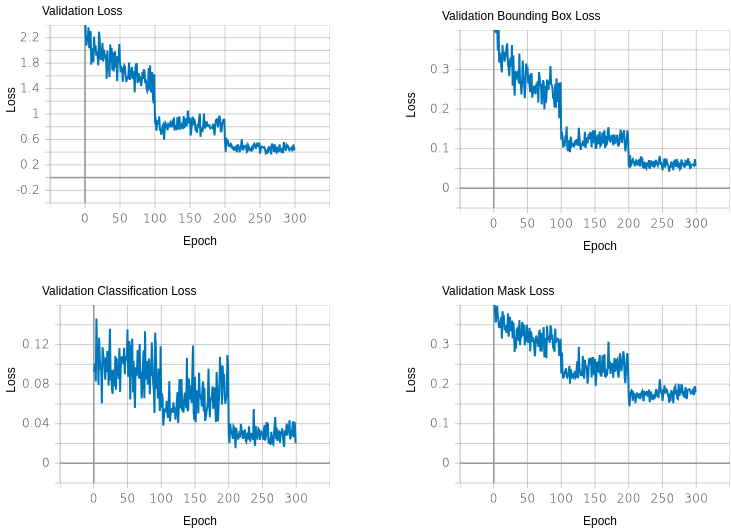
\includegraphics[scale=0.36]{gambar/resnet50-val.png}
	\caption{Grafik Perubahan \textit{Validation Loss} pada Resnet-50}
	\label{fig:resnet50-val}
\end{figure}

Selain menggunakan \textit{Loss Function} untuk mengukur peforma hasil \textit{training} yang sudah dilakukan, digunakan juga \textit{mean Average Precision (mAP)}. \textit{Precision} sendiri merupakan fungsi untuk menggambarkan tingkat keakuratan antara data yang diminta dengan hasil prediksi yang diberikan oleh model. Maka, \textit{precision} merupakan rasio prediksi benar positif (TP) dibandingkan dengan keseluruhan hasil yang diprediksi positif (TP dan FP). Rumus untuk mencari \textit{Precision} adalah sebagai berikut :
\begin{equation}
	Precision = \frac{TP}{TP+FP} 
\end{equation}

Perhitungan \textit{mAP} pada penelitian ini dilakukan setiap 5 \textit{epoch} sekali, karena jika dilakukan setiap \textit{epoch} akan memerlukan \textit{training time} yang lebih lama serta \textit{resource hardware} yang diperlukan lebih besar. Nilai \textit{mAP} tertinggi didapatkan pada \textit{epoch} ke 220 sebesar 94.92. Gambar \ref{fig:resnet50-map} merupakan grafik yang menunjukan perubahan \textit{validation mean Average Precision} dari \textit{epoch} 1 sampai 300. 

\begin{figure}[h]
	\centering
	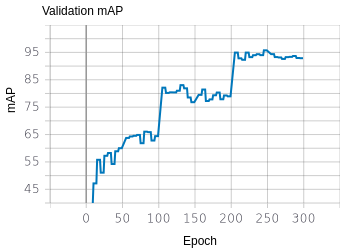
\includegraphics[scale=0.4]{gambar/resnet50-map.png}
	\caption{Grafik Perubahan \textit{Validation mAP} pada Resnet-50}
	\label{fig:resnet50-map}
\end{figure}

\newpage

\subsection{Resnet-101}
\label{subsec:resnet101}

Tabel \ref{tab:conf-resnet101} merupakan parameter-parameter yang digunakan untuk membuat model Mask R-CNN dengan menggunakan \textit{backbone} Resnet-101.

\begin{longtable}[h]{|l|l|}
	\hline
	\multicolumn{2}{|c|}{\textbf{Pengaturan Model Resnet-101}}                                                                                                                                                                         \\ \hline
	BACKBONE                        & resnet101                                                                                                                                                                              \\ \hline
	BACKBONE\_STRIDES               & {[}4, 8, 16, 32, 64{]}                                                                                                                                                                 \\ \hline
	BATCH\_SIZE                     & 1                                                                                                                                                                                      \\ \hline
	BBOX\_STD\_DEV                  & {[}0.1 0.1 0.2 0.2{]}                                                                                                                                                                  \\ \hline
	COMPUTE\_BACKBONE\_SHAPE        & None                                                                                                                                                                                   \\ \hline
	DETECTION\_MAX\_INSTANCES       &	 50                                                    	\\ \hline
	IMAGE\_META\_SIZE               & 16                                                                                                                                                                                     \\ \hline
	IMAGE\_MIN\_DIM                 & 400                                                                                                                                                                                    \\ \hline
	IMAGE\_MIN\_SCALE               & 0                                                                                                                                                                                      \\ \hline
	IMAGE\_RESIZE\_MODE             & square                                                                                                                                                                                 \\ \hline
	IMAGE\_SHAPE                    & {[}512 512{]}                                                                                                                                                                             \\ \hline
	LEARNING\_MOMENTUM              & 0.9                                                                                                                                                                                    \\ \hline
	LEARNING\_RATE                  & 0.001                                                                                                                                                                                  \\ \hline
	LOSS\_WEIGHTS                   & \begin{tabular}[c]{@{}l@{}}\{'rpn\_class\_loss': 1.0, \\ 'rpn\_bbox\_loss': 1.0, \\ 'mrcnn\_class\_loss': 1.0, \\ 'mrcnn\_bbox\_loss': 1.0, \\ 'mrcnn\_mask\_loss': 1.0\}\end{tabular} \\ \hline
	MASK\_POOL\_SIZE                & 14                                                                                                                                                                                     \\ \hline
	MASK\_SHAPE                     & {[}28, 28{]}                                                                                                                                                                           \\ \hline
	MAX\_GT\_INSTANCES              & 50                                                                                                                                                                                     \\ \hline
	MEAN\_PIXEL                     & {[}123.7 116.8 103.9{]}                                                                                                                                                                \\ \hline
	MINI\_MASK\_SHAPE               & (56, 56)                                                                                                                                                                               \\ \hline
	NAME                            & object                                                                                                                                                                                 \\ \hline
	NUM\_CLASSES                    & 4                                                                                                                                                                                      \\ \hline
	POOL\_SIZE                      & 7                                                                                                                                                                                      \\ \hline
	MASK\_SHAPE                     & {[}28, 28{]}                                                                                                                                                                           \\ \hline
	MAX\_GT\_INSTANCES              & 50                                                                                                                                                                                     \\ \hline
	MEAN\_PIXEL                     & {[}123.7 116.8 103.9{]}                                                                                                                                                                \\ \hline
	MINI\_MASK\_SHAPE               & (56, 56)                                                                                                                                                                               \\ \hline
	NAME                            & object                                                                                                                                                                                 \\ \hline
	NUM\_CLASSES                    & 4                                                                                                                                                                                      \\ \hline
	POOL\_SIZE                      & 7                                                                                                                                                                                      \\ \hline
	POST\_NMS\_ROIS\_INFERENCE      & 1000                                                                                                                                                                                   \\ \hline
	POST\_NMS\_ROIS\_TRAINING       & 2000                                                                                                                                                                                   \\ \hline
	PRE\_NMS\_LIMIT                 & 6000                                                                                                                                                                                   \\ \hline
	ROI\_POSITIVE\_RATIO            & 0.33                                                                                                                                                                                   \\ \hline
	RPN\_ANCHOR\_RATIOS             & {[}0.5, 1, 2{]}                                                                                                                                                                        \\ \hline
	RPN\_ANCHOR\_SCALES             & (32, 64, 128, 256, 512)                                                                                                                                                                \\ \hline
	RPN\_ANCHOR\_STRIDE             & 1                                                                                                                                                                                      \\ \hline
	RPN\_BBOX\_STD\_DEV             & {[}0.1 0.1 0.2 0.2{]}                                                                                                                                                                  \\ \hline
	RPN\_NMS\_THRESHOLD             & 0.7                                                                                                                                                                                    \\ \hline
	RPN\_TRAIN\_ANCHORS\_PER\_IMAGE & 256                                                                                                                                                                                    \\ \hline
	STEPS\_PER\_EPOCH               & 100                                                                                                                                                                                    \\ \hline
	TOP\_DOWN\_PYRAMID\_SIZE        & 256                                                                                                                                                                                    \\ \hline
	TRAIN\_BN                       & False                                                                                                                                                                                  \\ \hline
	TRAIN\_ROIS\_PER\_IMAGE         & 200                                                                                                                                                                                    \\ \hline
	USE\_MINI\_MASK                 & True                                                                                                                                                                                   \\ \hline
	USE\_RPN\_ROIS                  & True                                                                                                                                                                                   \\ \hline
	VALIDATION\_STEPS               & 30                                                                                                                                                                                     \\ \hline
	WEIGHT\_DECAY                   & 0.0001  
	\\ \hline 
	\caption{Konfigurasi Model menggunakan Resnet-101 }
	\label{tab:conf-resnet101}
\end{longtable}

Setelah dilakukan serangkaian proses training yang memakan waktu sekitar 4 jam 9 menit 16 detik didapatkan \textit{output} berupa \textit{model file}  dengan format \textit{h5} yang mempunyai ukuran 244 MB. \textit{Training loss} terendah yang berhasil dicapai dengan menggunakan \textit{backbone} Resnet-101 (pada \textit{epoch} ke 244) adalah 0.3933 dengan rincian \textit{training bounding box loss} sebesar 0.04164, \textit{training classification loss} sebesar 0.0247 serta \textit{training mask loss} sebesar 0.1403. Namun untuk \textit{training bounding box loss} terendah terdapat pada \textit{epoch} ke 246 dengan nilai sebesar 0.04083, \textit{training classification loss} terendah pada \textit{epoch} ke 234 dengan nilai 0.01957. Gambar \ref{fig:resnet101-training} merupakan grafik yang menunjukkan perubahan \textit{training loss, training bounding box loss, training classification loss,} serta \textit{training mask loss} dari \textit{epoch} 1 sampai 300. 

\begin{figure}[h]
	\centering
	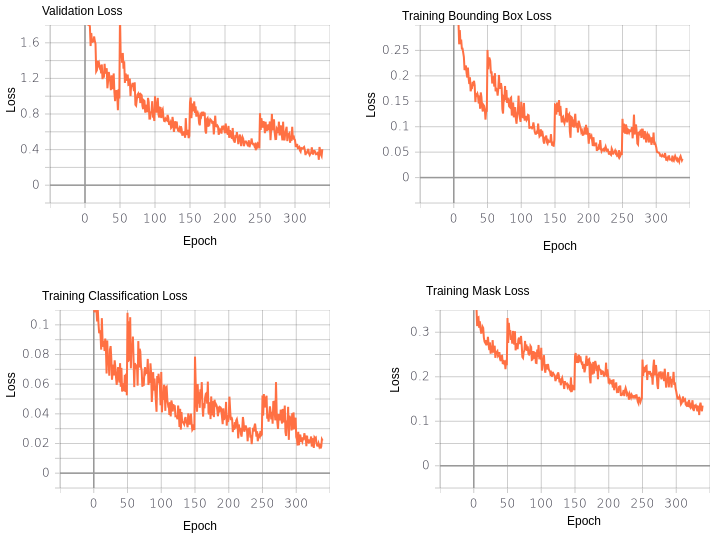
\includegraphics[scale=0.36]{gambar/resnet101-training.png}
	\caption{Grafik Perubahan \textit{Training Loss} pada Resnet-101}
	\label{fig:resnet101-training}
\end{figure}

Sedangkan pada saat proses \textit{validation} sendiri \textit{Loss} terendah yang berhasil dicapai pada \textit{epoch} ke 266 dengan nilai sebesar 0.299 dengan rincian \textit{validation bounding box loss} sebesar 0.03867, \textit{validation classification loss} sebesar 0.01246 serta \textit{validation mask loss} sebesar 0.1461. Gambar \ref{fig:resnet101-val} merupakan grafik yang menunjukkan perubahan \textit{validation loss, validation bounding box loss, validation classification loss,} serta \textit{validation mask loss} dari \textit{epoch} 1 sampai 300.

\begin{figure}[h]
	\centering
	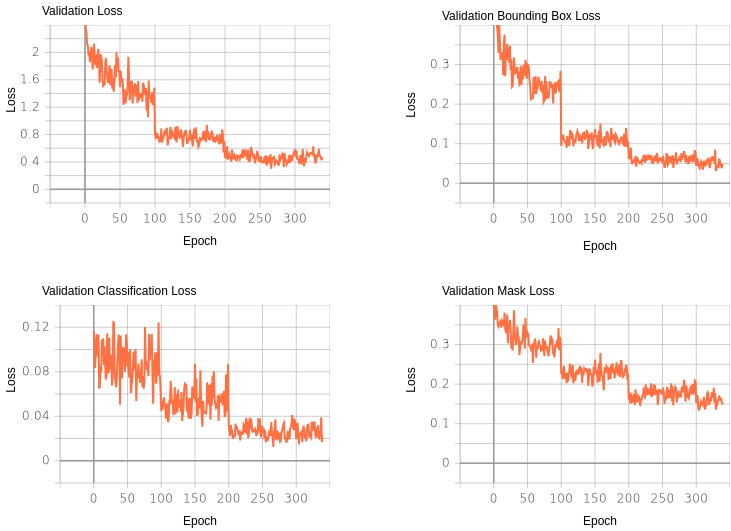
\includegraphics[scale=0.36]{gambar/resnet101-val.png}
	\caption{Grafik Perubahan \textit{Validation Loss} pada Resnet-101}
	\label{fig:resnet101-val}
\end{figure}

Nilai \textit{mAP} tertinggi didapatkan pada \textit{epoch} ke 215 sebesar 96.21. Gambar \ref{fig:resnet101-map} merupakan grafik yang menunjukan perubahan \textit{validation mean Average Precision} dari \textit{epoch} 1 sampai 300.

\begin{figure}[h]
	\centering
	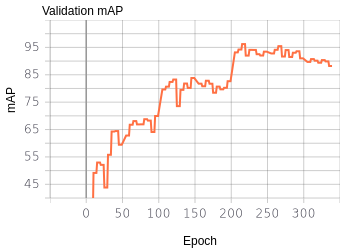
\includegraphics[scale=0.4]{gambar/resnet101-map.png}
	\caption{Grafik Perubahan \textit{Validation mAP} pada Resnet-101}
	\label{fig:resnet101-map}
\end{figure} 

\newpage

\subsection{MobileNet-V1}
\label{subsec:mobilenetv1}

Tabel \ref{tab:conf-mobilenet-v1} merupakan parameter-parameter yang digunakan untuk membuat model Mask R-CNN dengan menggunakan \textit{backbone} Mobilenet-V1.

\begin{longtable}[h]{|l|l|}
	\hline
	\multicolumn{2}{|c|}{\textbf{Pengaturan Model Mobilenet-V1}}                                                                                                                                                                         \\ \hline
	BACKBONE                        & mobilenetv1                                                                                                                                                                              \\ \hline
	BACKBONE\_STRIDES               & {[}2, 4, 8, 16, 32{]}                                                                                                                                                                 \\ \hline
	BATCH\_SIZE                     & 1                                                                                                                                                                                      \\ \hline
	BBOX\_STD\_DEV                  & {[}0.1 0.1 0.2 0.2{]}                                                                                                                                                                  \\ \hline
	COMPUTE\_BACKBONE\_SHAPE        & None                                                                                                                                                                                   \\ \hline
	DETECTION\_MAX\_INSTANCES       &	 50                                                    	\\ \hline
	IMAGE\_META\_SIZE               & 16                                                                                                                                                                                     \\ \hline
	IMAGE\_MIN\_DIM                 & 400                                                                                                                                                                                    \\ \hline
	IMAGE\_MIN\_SCALE               & 0                                                                                                                                                                                      \\ \hline
	IMAGE\_RESIZE\_MODE             & square                                                                                                                                                                                 \\ \hline
	IMAGE\_SHAPE                    & {[}512 512{]}                                                                                                                                                                             \\ \hline
	LEARNING\_MOMENTUM              & 0.9                                                                                                                                                                                    \\ \hline
	LEARNING\_RATE                  & 0.001                                                                                                                                                                                  \\ \hline
	LOSS\_WEIGHTS                   & \begin{tabular}[c]{@{}l@{}}\{'rpn\_class\_loss': 1.0, \\ 'rpn\_bbox\_loss': 1.0, \\ 'mrcnn\_class\_loss': 1.0, \\ 'mrcnn\_bbox\_loss': 1.0, \\ 'mrcnn\_mask\_loss': 1.0\}\end{tabular} \\ \hline
	MASK\_POOL\_SIZE                & 14                                                                                                                                                                                     \\ \hline
	MASK\_SHAPE                     & {[}28, 28{]}                                                                                                                                                                           \\ \hline
	MAX\_GT\_INSTANCES              & 50                                                                                                                                                                                     \\ \hline
	MEAN\_PIXEL                     & {[}123.7 116.8 103.9{]}                                                                                                                                                                \\ \hline
	MINI\_MASK\_SHAPE               & (56, 56)                                                                                                                                                                               \\ \hline
	NAME                            & object                                                                                                                                                                                 \\ \hline
	NUM\_CLASSES                    & 4                                                                                                                                                                                      \\ \hline
	POOL\_SIZE                      & 7                                                                                                                                                                                      \\ \hline
	MASK\_SHAPE                     & {[}28, 28{]}                                                                                                                                                                           \\ \hline
	MAX\_GT\_INSTANCES              & 50                                                                                                                                                                                     \\ \hline
	MEAN\_PIXEL                     & {[}123.7 116.8 103.9{]}                                                                                                                                                                \\ \hline
	MINI\_MASK\_SHAPE               & (56, 56)                                                                                                                                                                               \\ \hline
	NAME                            & object                                                                                                                                                                                 \\ \hline
	NUM\_CLASSES                    & 4                                                                                                                                                                                      \\ \hline
	POOL\_SIZE                      & 7                                                                                                                                                                                      \\ \hline
	POST\_NMS\_ROIS\_INFERENCE      & 1000                                                                                                                                                                                   \\ \hline
	POST\_NMS\_ROIS\_TRAINING       & 2000                                                                                                                                                                                   \\ \hline
	PRE\_NMS\_LIMIT                 & 6000                                                                                                                                                                                   \\ \hline
	ROI\_POSITIVE\_RATIO            & 0.33                                                                                                                                                                                   \\ \hline
	RPN\_ANCHOR\_RATIOS             & {[}0.5, 1, 2{]}                                                                                                                                                                        \\ \hline
	RPN\_ANCHOR\_SCALES             & (32, 64, 128, 256, 512)                                                                                                                                                                \\ \hline
	RPN\_ANCHOR\_STRIDE             & 1                                                                                                                                                                                      \\ \hline
	RPN\_BBOX\_STD\_DEV             & {[}0.1 0.1 0.2 0.2{]}                                                                                                                                                                  \\ \hline
	RPN\_NMS\_THRESHOLD             & 0.7                                                                                                                                                                                    \\ \hline
	RPN\_TRAIN\_ANCHORS\_PER\_IMAGE & 256                                                                                                                                                                                    \\ \hline
	STEPS\_PER\_EPOCH               & 100                                                                                                                                                                                    \\ \hline
	TOP\_DOWN\_PYRAMID\_SIZE        & 256                                                                                                                                                                                    \\ \hline
	TRAIN\_BN                       & False                                                                                                                                                                                  \\ \hline
	TRAIN\_ROIS\_PER\_IMAGE         & 200                                                                                                                                                                                    \\ \hline
	USE\_MINI\_MASK                 & True                                                                                                                                                                                   \\ \hline
	USE\_RPN\_ROIS                  & True                                                                                                                                                                                   \\ \hline
	VALIDATION\_STEPS               & 30                                                                                                                                                                                     \\ \hline
	WEIGHT\_DECAY                   & 0.0001  
	\\ \hline 
	\caption{Konfigurasi Model menggunakan Mobilenet-V1 }
	\label{tab:conf-mobilenet-v1}
\end{longtable}

\newpage

Setelah dilakukan serangkaian proses training yang memakan waktu sekitar 3 jam 18 menit 44 detik didapatkan \textit{output} berupa \textit{model file}  dengan format \textit{h5} yang mempunyai ukuran 83.3 MB. \textit{Training loss} terendah yang berhasil dicapai dengan menggunakan \textit{backbone} Mobilenet-V1 (pada \textit{epoch} ke 46) adalah 1.604 dengan rincian \textit{training bounding box loss} sebesar 0.2322, \textit{training classification loss} sebesar 0.07858 serta \textit{training mask loss} sebesar 0.6729. Namun untuk \textit{training bounding box loss} terendah terdapat pada \textit{epoch} ke 48 dengan nilai sebesar 0.2239, \textit{training classification loss} terendah pada \textit{epoch} ke 61 dengan nilai 0.06219 serta \textit{training mask loss} terendah pada \textit{epoch} ke 61 sebesar 0.5701. Gambar \ref{fig:mobilenet-training} merupakan grafik yang menunjukkan perubahan \textit{training loss, training bounding box loss, training classification loss,} serta \textit{training mask loss} dari \textit{epoch} 1 sampai 300. 

\begin{figure}[h]
	\centering
	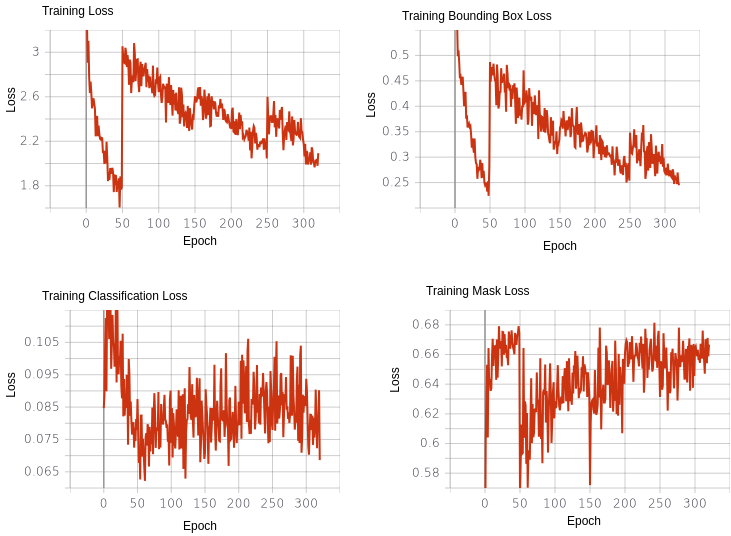
\includegraphics[scale=0.36]{gambar/mobilenetv1-train.png}
	\caption{Grafik Perubahan \textit{Training Loss} pada Mobilenet-V1}
	\label{fig:mobilenetv1-training}
\end{figure}


Sedangkan pada saat proses \textit{validation} sendiri \textit{Loss} terendah yang berhasil dicapai pada \textit{epoch} ke 281 dengan nilai sebesar 1.624 dengan rincian \textit{validation bounding box loss} sebesar 0.2088, \textit{validation classification loss} sebesar 0.04799 serta \textit{validation mask loss} sebesar 0.6001. Namun untuk \textit{validation bounding box loss} terendah berada pada \textit{epoch} ke 300 dengan nilai sebesar 0.1927 sedangkan \textit{validation classification loss} terendah pada \textit{epoch} ke 70 dengan nilai 0.02607 serta \textit{validation mask loss} terendah pada \textit{epoch} ke 295 dengan nilai 0.5625. Gambar \ref{fig:mobilenetv1-val} merupakan grafik yang menunjukkan perubahan \textit{validation loss, validation bounding box loss, validation classification loss,} serta \textit{validation mask loss} dari \textit{epoch} 1 sampai 300.

\begin{figure}[h]
	\centering
	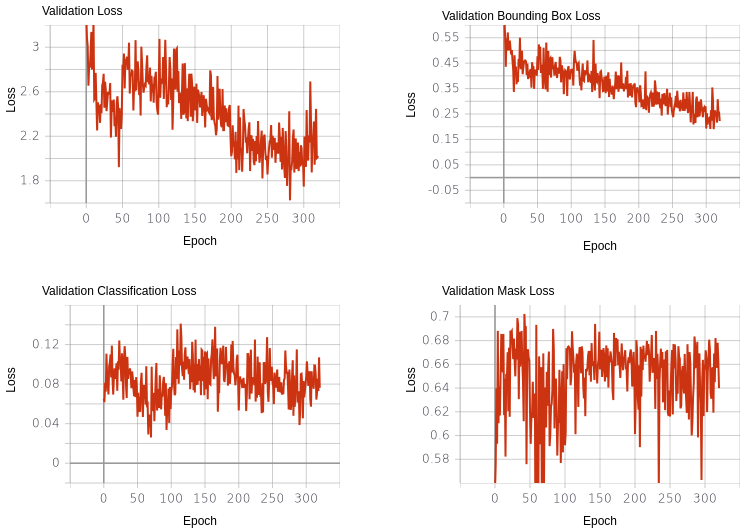
\includegraphics[scale=0.36]{gambar/mobilenetv1-val.png}
	\caption{Grafik Perubahan \textit{Validation Loss} pada Mobilenet-V1}
	\label{fig:mobilenetv1-val}
\end{figure}

Nilai \textit{mAP} tertinggi didapatkan pada \textit{epoch} ke 210 sebesar 26.04. Gambar \ref{fig:mobilenetv1-map} merupakan grafik yang menunjukan perubahan \textit{validation mean Average Precision} dari \textit{epoch} 1 sampai 300.

\newpage

\begin{figure}[h]
	\centering
	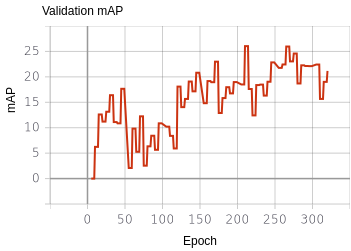
\includegraphics[scale=0.4]{gambar/mobilenetv1-map.png}
	\caption{Grafik Perubahan \textit{Validation mAP} pada Mobilenet-V1}
	\label{fig:mobilenetv1-map}
\end{figure} 

Tabel \ref{tab:train-recap} adalah tabel perbandingan dari \textit{output file size} dan \textit{mAP} dari total 3 model dengan \textit{backbone} berbeda yang diuji. Tahap ini masih merupakan hasil tahap \textit{training}. Sedangkan Gambar \ref{fig:graph-recap} merupakan grafik perbandingan \textit{mAP} dengan \textit{file size}. Proses selanjutnya setelah mendapatkan hasil yang ditunjukkan pada setiap model adalah melakukan proses prediksi atau melakukan \textit{testing data}.

\begin{table}[h]
	\centering
	\begin{tabular}{|c|l|l|l|}
		\hline
		\textbf{No.} & \multicolumn{1}{c|}{\textit{\textbf{Backbone}}} & \multicolumn{1}{c|}{\textit{\textbf{Output File Size}}} & \multicolumn{1}{c|}{\textbf{mAP}} \\ \hline
		1            & Resnet-50                                       & 170.9 MB                                                & 94.92\%                           \\ \hline
		2            & Resnet-101                                      & 244 MB                                                  & 96.21\%                           \\ \hline
		3            & Mobilenet-V1                                    & 83.3 MB                                                 & 26.04\%                           \\ \hline
	\end{tabular}
	\caption{Tabel Perbandingan Model dengan \textit{backbone} yang berbeda}
	\label{tab:train-recap}
\end{table}

\newpage

\begin{figure}[h]
	\centering
	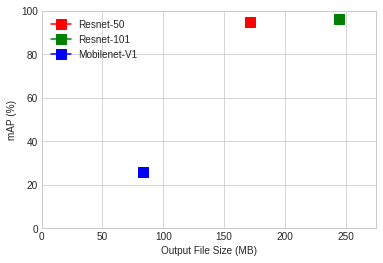
\includegraphics[scale=0.75]{gambar/graph-recap.png}
	\caption{Grafik Perbandingan Model dengan \textit{backbone} yang berbeda}
	\label{fig:graph-recap}
\end{figure}